\documentclass[11pt]{article}
\usepackage[margin=0.85in]{geometry}
\usepackage{amsmath,amssymb,graphicx,hyperref}
\setlength{\parindent}{0pt}\setlength{\parskip}{6pt}
\setlength{\emergencystretch}{3em}
\begin{document}
{\Large Single-target batch floor in the declared m8 model}\\
November 13, 2026. Unsigned producer evidence [pcc:unverified].

\textbf{Scope.} This corrects one incoming entropy-charge cost projection.
It is not a lower bound on an actual sparse solver or ECDLP, and it does not
close PKM or another encoding.

Let $H_2$ denote binary entropy and $\theta_8=8H_2(1/8)$. Exact Lean bounds give
\[
 \theta_8=24-7\frac{\log7}{\log2},\qquad4<\theta_8<5.
\]
The incoming unclamped exponent and its balanced whole-attack call exponent obey
\[
 \frac25<\frac2{9-\theta_8}<\frac12,\qquad
 1-\frac7{9-\theta_8}<0.
\]
The apparent gain is paired with fewer than one total solver call. Even allowing
all useful outputs per call, enforce the optimistic single-target batch floor:
\[
 W(p,b,c)=\max\{1,p/b^7\}\,c+b^2,\quad p>1,\ b\ge1,\ c\ge b^4.
\]
The declared charge $c=b^{\theta_8}$ meets that bound. Lean establishes
\[
                 p<W(p,b,b^{\theta_8})^2\quad\text{for every }p>1,b\ge1.
\]
No wall time, GAE, measured solver exponent or universal cryptographic bound
is asserted.

\textbf{Proof.} For charged work $t$, the model implies $b^4\le t$ and
$p\le tb^3$. If $b>1$, then $p<pb\le tb^4\le t^2$.
If $b=1$, then $t\ge p>1$, so $t^2>p$. The central surplus identity is
\[
 (tb^3-p)b+(t-b^4)t=t^2-pb.
\]
The entropy bounds use the exact inequalities $2^{19}<7^7<2^{20}$.

\begin{center}
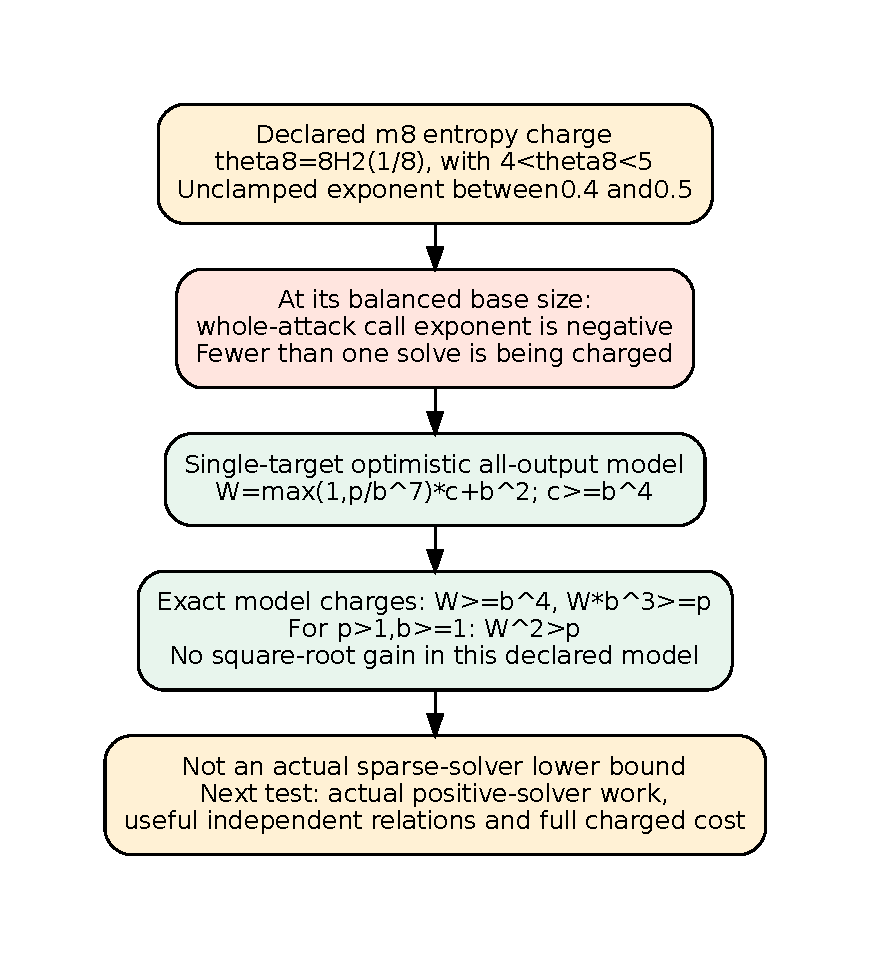
\includegraphics[width=0.9\linewidth,height=0.34\textheight,keepaspectratio]{floor.pdf}
\end{center}

\newpage
{\Large Evidence scope and the corrected next test}

\textbf{What the review changes.} The D8,3 cell is still a degree diagnostic;
its result alone does not decide the advertised single-target gain under this
charge model. Actual sparse solver work may be lower than the dense proxy.
Measure positive-solver work, witness extraction, actual solve count and useful
independent relations before selecting an expensive new run. A fixed exponent
below1/2 is still exponential in input bits; the original objective requires
a uniform growing-parameter bit-cost bound.

\textbf{Bounded source observations.} Incoming snapshot
\path{5965fa03b}. L1's generator explicitly enforces rational targets; its
hash matches the manifest. Its level9 closure is censored; an F4 degree10
trace is distinct from the frozen completed-closure condition. The L1 manifest
names closure Rust files absent from the inspected committed study listing;
replay-source recovery remains open. L2 itself limits truncated ideal searches.
L3's checker distinguishes unsplit degrees from alternate encodings and
full-space size from actual solver cost. L4's checker flags success conditioning
and mask/filter scope. L5's point-ordered widths do not exclude arbitrary
algebraic/interleaved representations. These are source observations, not
independent numerical replays or a blanket closure. Full original protocol
and code review of all five leads is unfinished.

\textbf{Formal map.} \path{PrimeICCostFloor.lean}, frozen source
\path{d42ef1874}. Twelve declarations cover the universal surplus, explicit
charge inequalities, actual defined work expression, exact entropy formula
and bounds, unclamped exponents and corrected entropy work. Exact hypotheses
and declaration bindings are linked from the Markdown report. All producer
PCC standing is unsigned.

\textbf{Checks.} Lean4.35.0 with unchanged pinned dependencies. Build003
passes2074 jobs. Full tracked-source audit155 declarations, zero failing and
zero extra trusted axioms; fresh import-inclusive completion has its own
receipt. Standard foundations only. Build001 had power-rewrite/positivity
proof issues; build002 corrects them and build003 adds exact exponent bounds.
Failed and completed logs are retained; earlier source hashes are unchanged.

Native record \path{IDC1h0f32be38dee24607} checks only the universal surplus
identity at32+32 points using the unchanged checker and exact universal source.
It does not execute Lean or prove inequalities, logarithms or actual solver
cost. Its adapter's22 inherited tests pass. No runtime claim.

\textbf{Next protocol.} Recover pinned native source; separate the degree
cell from actual relation finding on online masked targets. Charge at least one
whole solve, base generation, rejected candidates, useful independent output,
linear algebra and final scalar verification. Retain controls/censoring and
isolate hosts for time comparisons. Kummer eligibility $2^t\mid p-1$ and all
symmetry/bit costs must be explicit. The draft is not executed: isolab monthly
budget is exhausted. No new paid job, benchmark, leaderboard or ecdb edit.

\textbf{Sources.} Exact incoming L1 protocol/amendments/verdict/generator;
L2 report, L3/L4 checker reports and L5 report; Galbraith15.8.1--2 from the
previous source-pinned author-hosted book; pinned logarithm/power/inequality
APIs. KB/conductor unavailable, bounded fallback; no priority claim for elementary
batch accounting. Editable DOT/SVG and source-linked report/evidence accompany
this PDF.
\end{document}
